\chapter{Необходимые сведения о сетях}

\section{Эталонные модели}
В теории компьютерных сетей выделяют две эталонные модели архитектуры: OSI и TCP/IP. Эти модели представляют собой деление сети на уровни, а также набор протоколов. Несмотря на то, что протоколы, связанные с эталонной моделью OSI, сейчас не ис­пользуются, сама модель до сих пор весьма актуальна. В эталонной модели TCP/IP все наоборот: сама модель сейчас почти не используется, а ее протоколы являются едва ли не самыми распространенными. В современной сети модели OSI и TCP/IP служат двум разным целям. Модель TCP/IP --- это модель реализации, поскольку она предоставляет руководство для тех, кто будет создавать сетевое оборудование или программное обеспечение, совместимое с TCP/IP. Модель OSI --- это, скорее, абстрактная модель, которую можно использовать для понимания широкого спектра сетевых архитектур. ~\cite{wt-computer-networks, severans}

\subsection{OSI}
Модель OSI состоит из семи уровней:
\begin{enumerate}
    \item Физический уровень занимается непосредственной передачей данных по каналу связи.
    \item Канальный уровень обеспечивает взаимодействие физического и сетевого уровней. Обнаруживает и корректирует ошибки передачи данных на физическом уровне от сетевого уровня, а также обеспечивает согласование скоростей в сети.
    \item Сетевой уровень занимается управлением операциями подсети, основной из которых является маршрутизация пакетов, то есть определение пути, по которому будет осуществляться пересылка пакетов. В случае высокой нагрузки происходит перестройка маршрута, из-за чего последовательные пакеты могут идти по сети разными путями и приходить адресату в разнобой.
    \item Транспортный уровень является прослойкой между сеансовым и сетевым уровнями. Обеспечивает правильную доставку данных, а также изолирует более высокие уровни от каких-либо изменений в аппаратной технологии с течением времени.
    \item Сеансовый уровень позволяет пользователям различных устройств устанавливать сеансы связи друг с другом. При этом предоставляются различные типы сервисов, среди которых:
    \begin{itemize}
        \item управление диалогом --- отслеживание очередности передачи данных;
        \item управление маркерами --- предотвращение одновременного выполнения критичной операции несколькими системами;
        \item синхронизация --- установка служебных меток внутри длинных сообщений, позволяющих продолжить передачу с того места, на котором она оборвалась, даже после сбоя и восстановления.
    \end{itemize}
    \item Уровень представления занимается по большей части синтаксисом и семантикой передаваемой информации. Преобразует различные внутренние представления данных в стандартизированный вид, тем самым предоставляя возможность определения и изменения структур данных более высокого уровня. Для повышения эффективности обмена текстами и графическими изображениями уровень представления может оказывать услуги по сжатию/распаковке информации. К функциям уровня представления относится также кодирование графических изображений,
    аудио и видео в соответствии с различными стандартами, например JPEG, MPEG, TIFF.~\cite{olipher}
    \item Прикладной уровень --- уровень, на котором функционируют приложения. Также к этому уровню относится большая часть известных протоколов передачи данных, таких как HTTP, FTP, SMTP, DNS.
\end{enumerate}

\subsection{TCP/IP}
В отличии от OSI, архитектура TCP/IP состоит из четырёх уровней:
\begin{enumerate}
    \item Канальный уровень можно считать объединением физического и канального уровней модели OSI.
    \item Межсетевой уровень, или уровень IP, соответствует сетевому уровню модели OSI. На этом уровне вводится протокол IP с дополнительным протоколом ICMP (Internet Control Message Protocol, интернет протокол управления сообщений), использующимся, например, в утилите traceroute.
    \item Транспортный уровень объединяет в себе транспортный и сеансовый уровни модели OSI. Протоколы этого уровня будут рассмотрены в следующем параграфе. Далее в работе сеансовый уровень будет выделяться в рамках модели TCP/IP между транспортным и прикладным уровнями.
    \item Прикладной уровень объединяет в себе уровень представления и прикладной уровень модели OSI.
\end{enumerate}

В сети Интернет используются две версии протокола IP: IPv4 и IPv6. В начале восьмидесятых --- на момент изобретения IPv4 --- считалось, что Интернет будут использовать лишь университеты, правительство, крупные компании, поэтому создатели сети посчитали, что $2^{32}$ (более четырёх миллиардов, на деле в адресации участвует примерно на четверть меньше) адресов должно хватить. Однако уже через десять лет стало ясно, что четырёх миллиардов адресов мало, и появилась потребность расширять сеть. С разницей в два года появились два решения: Network Address Translator (NAT, май 1994-го) и IPv6 (декабрь 1995-го). 

NATs создали новую проблему: предполагалось, что каждая машина, подключённая к сети, должна иметь возможность связаться с любой другой машиной сети напрямую; NATs же логически ввели концепцию локальных сетей в рамках сети Интернет и, как следствие, публичные и приватные адреса. Теперь можно было выдавать адрес не каждому устройству, а целой группе устройств. Более того, публичные адреса можно экономить и другим способом: при отключении локальной сети от глобальной, её публичный адрес передавался другой сети --- динамическая адресация. Однако теперь пропала возможность прямой связи двух хостов, что затрудняет разработку peer-to-peer приложений. Более подробно эта проблема будет разобрана в \ref{ya:nat_traversal}.

IPv6 имеет уже $2^{128}$ адресов, что решает проблему нехватки адресов (и позволяет хорошо работать peer-to-peer приложениям), однако имеет свои недостатки\footnote{habr.com: \href{https://habr.com/en/companies/droider/articles/568778/}{Что такое и зачем нужен IPv6?} (\url{shorturl.at/iSW03})}.

\section{Транспортные протоколы}
В Интернете нашли своё применение два основных протокола транспортного уровня, один из которых требует установления соединения, другой --- нет. Эти протоколы дополняют друг друга. Протоколом без установления соединения является UDP, не делающий практически ничего, кроме отправки пакетов между приложениями, позволяя последним надстраивать свои собственные протоколы. Протоколом с установлением соединения является TCP, обеспечивающий надежность сети, выполняя повторную передачу данных, а также осуществляет управление потоком данных и контроль перегрузки --- и все это от лица приложений, которые его используют.

В следующих разделах мы рассмотрим TCP и UDP, а также протокол QUIC, формально не считающийся протоколом транспортного уровня, так как является надстройкой над UDP.

\subsection{TCP}
Протокол TCP (Transmission Control Protocol --- протокол управления передачей) был специально разработан для обеспечения надежного сквозного байтового потока по ненадежной сети. Объединенная сеть отличается от отдельной сети тем, что её различные участки могут обладать сильно различающейся топологией, пропускной способностью, значениями времени задержки, размерами пакетов и другими параметрами. При разработке TCP основное внимание уделялось способности протокола
адаптироваться к свойствам объединенной сети и отказоустойчивости при возникновении различных проблем.~\cite{wt-computer-networks}

В рамках работы нас будет интересовать лишь две характеристики протокола: способность сохранять целостность данных, то есть доставлять все пакеты и восстанавливать их последовательность, и установка логического соединения в небезопасной сети. Для решения задачи сохранения целостности данных используются порядковые номера пакетов, а также накопительное подтверждение получения пакетов. Эту возможность обеспечивает схема двойного рукопожатия (показаны синим на рисунках \ref{fig:tcptls12}, \ref{fig:tcptls13}), используемая для синхронизации состояния отправителя и получателя.~\cite{wt-computer-networks} 

Безопасность соединения обеспечивает протокол TLS (Transport Layer Secu\-rity). TLS использует асимметричное шифрование для аутентификации, симметричное шифрование для конфиденциальности и коды аутентичности сообщений для сохранения целостности сообщений\footnote{\url{https://ru.wikipedia.org/wiki/TLS}}. На данный момент используются две версии: TLS1.2 (использует два цикла связи, показано бежевым на рисунке \ref{fig:tcptls12}), TLS1.3 (использует один цикл связи, показано бежевым на рисунке \ref{fig:tcptls13}).

\begin{figure}[h]
    \centering
    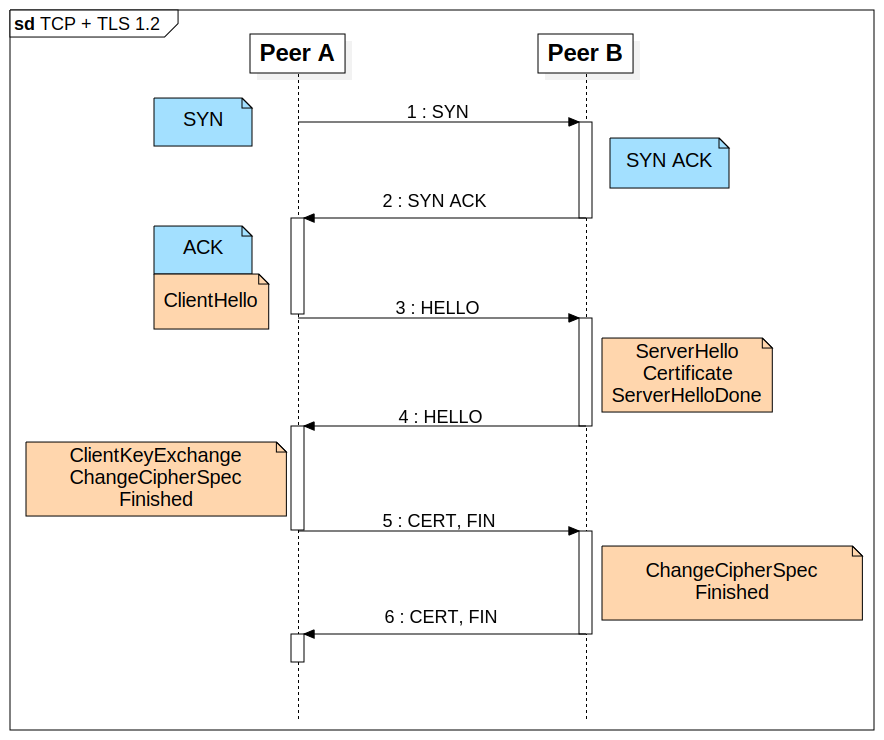
\includegraphics[width=0.8\textwidth]{TCP_TLS_1.2.pdf}
    \caption{Схема установки соединения TCP с использованием TLS 1.2}
    \label{fig:tcptls12}
\end{figure}

\begin{figure}[h]
    \centering
    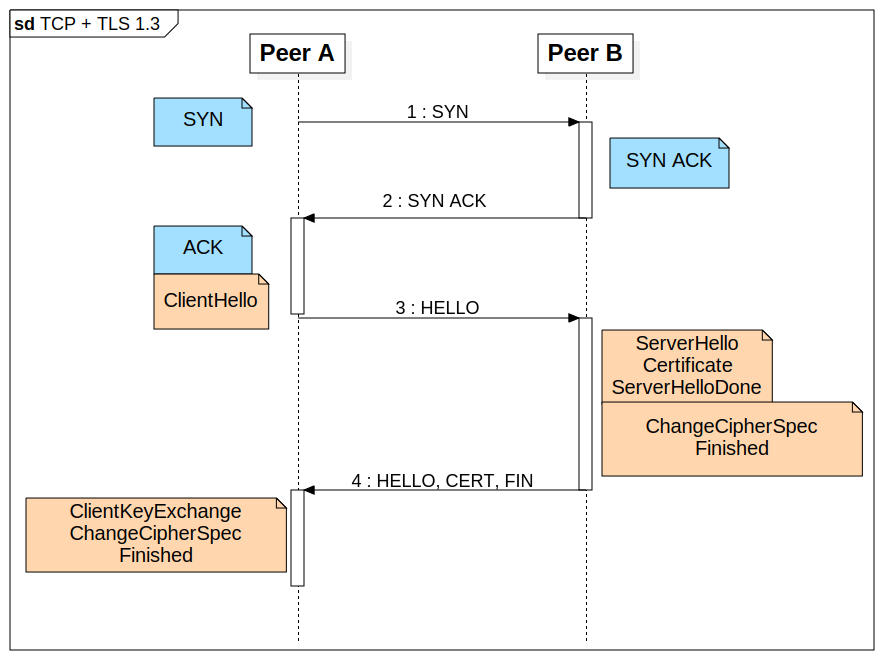
\includegraphics[width=0.8\textwidth]{TCP_TLS_1.3.pdf}
    \caption{Схема установки соединения TCP с использованием TLS 1.3}
    \label{fig:tcptls13}
\end{figure}

Поверх протокола TCP построены протоколы прикладного уровня, требующие передачу данных без потерь, например FTP, SMTP и HTTP.

\subsection{UDP}
В отличие от TCP, в UDP не предусмотрен контроль доставки пакетов. По сути происходит слепая пересылка данных без подтверждения от получателя. UDP используется в таких прикладных протоколах, как DNS (Domain Name System --- система доменных имён\footnote{\url{https://ru.wikipedia.org/wiki/DNS}}) и RPC (Remote Procedure Call -- вызов удалённой процедуры\footnote{\url{https://ru.wikipedia.org/wiki/Remote_procedure_call}}). 

Ввиду отсутствия гарантий целостности и безопасности передачи данных, заголовок UDP содержит лишь порты отправителя и получателя, размер пакета и контрольную сумму. Протокол также не устанавливает предварительное соединение. 

\subsection{QUIC}
Протокол QUIC (Quick UDP Internet Connections), как следует из названия, построен поверх протокола UDP. Протокол\footnote{\url{https://ru.wikipedia.org/wiki/QUIC}} был разработан компанией Google в 2013 году как альтернатива протоколу TCP с меньшей задержкой при установке соединения: синхронизация пакетов и настройка TLS происходит за один раунд (Рисунок \ref{fig:quic}).~\cite{quic}

\begin{figure}[h]
    \centering
    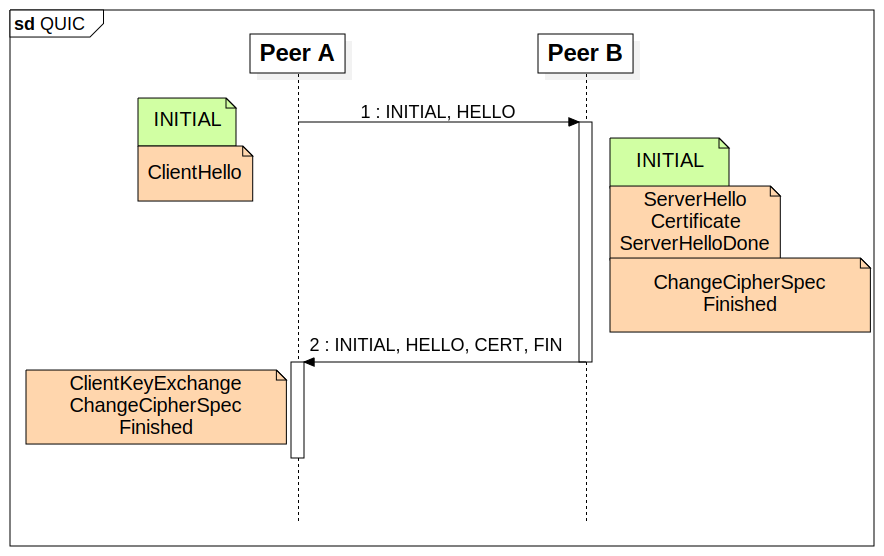
\includegraphics[width=0.8\textwidth]{QUIC.pdf}
    \caption{Схема установки соединения QUIC}
    \label{fig:quic}
\end{figure}

UDP в связке с QUIC используется в HTTP/3 по сравнению с TCP+TLS1.3 в HTTP/2.~\cite{dordalintroduction}

\section{Топологии сетей}
Сетевая топология --- это конфигурация графа, вершинам которого соответствуют конечные узлы сети (компьютеры и  маршрутизаторы), а рёбрам --- физические или информационные связи между вершинами.\footnote{\url{https://en.wikipedia.org/wiki/Network_topology}}

Далее будут представлены основные топологии сети. Обычно встречаются не отдельные топологии, а их комбинации.

\subsection{Полносвязная}
Топология, в которой каждое устройство непосредственно связано со всеми остальными устройствами в сети, то есть сообщения идут напрямую.
% \begin{figure}[h]
%     \centering
%     \includegraphics[width=0.5\textwidth]{fullyconn.pdf}
%     \caption{}
%     \label{fig:fullyconn}
% \end{figure}
\begin{figure}[h]
    \centering
    \includegraphics[width=0.4\textwidth]{fullyconn_clrd.pdf}
    \caption{}
    \label{fig:fullyconn}
\end{figure}

\subsection{Шина}
Топология, в которой каждое устройство подключено к общей магистрали. Сообщение пройдёт через каждое устройство, находящееся между отправителем и получателем.
% \begin{figure}[h]
%     \centering
%     \includegraphics[width=0.8\textwidth]{lineconn.pdf}
%     \caption{}
%     \label{fig:lineconn}
% \end{figure}
\begin{figure}[h]
    \centering
    \includegraphics[width=0.8\textwidth]{lineconn_clrd.pdf}
    \caption{}
    \label{fig:lineconn}
\end{figure}

\subsection{Звезда}
Каждое устройство в сети подключено к одному хабу, через который и происходит коммуникация. Далее в работе на месте хаба будет другое устройство сети, который выполняет роль хаба-маршрутизатора.
% \begin{figure}[h]
%     \centering
%     \includegraphics[width=0.5\textwidth]{starconn.pdf}
%     \caption{}
%     \label{fig:starconn}
% \end{figure}
\begin{figure}[h]
    \centering
    \includegraphics[width=0.4\textwidth]{starconn_clrd.pdf}
    \caption{}
    \label{fig:starconn}
\end{figure}

\subsection{Кольцо}
В данной топологии все устройства связаны в неразрывное кольцо. Эту топологию можно также представить как замкнутую "шину".
% \begin{figure}[h]
%     \centering
%     \includegraphics[width=0.5\textwidth]{ringconn.pdf}
%     \caption{}
%     \label{fig:ringconn}
% \end{figure}
\begin{figure}[h]
    \centering
    \includegraphics[width=0.4\textwidth]{ringconn_clrd.pdf}
    \caption{}
    \label{fig:ringconn}
\end{figure}
\newpage


\chapter{Yet Another P2P}
В рамках этой работы разрабатывается библиотека для развёртывания peer-to-peer сети на языке программирования Rust~\cite{chanda2018network, rustbook, programming-rust, rust-for-rustaceans}. Принципы построения сети в библиотеке отличаются от привычных, являются новаторскими. Вводится новая концепция пользователей в сети, а именно их возможности и принцип подключения к сети (\ref{ya:users}). Разработан протокол передачи сообщений в сети, построенный поверх UDP (\ref{ya:commprot}). Также библиотека предоставляет инструментарий для обеспечения надёжного шифрования симметричным алгоритмом (\ref{ya:security}).

\section{Пользователи сети}
\label{ya:users}
В современном мире у пользователей сети Интернет обычно имеется более одного устройства с доступом к Интернету. В библиотеке используются следующие концепции:

\begin{itemize}
    \item `Peer` --- уникальный пользователь сети;
    \item `Node` --- устройство пользователя, то есть каждый пользователь может иметь более одного устройства.
\end{itemize}

Пользователь в сети идентифицируется парой `PeerId` и именем пользователя, где `PeerId` --- 128-битный адрес, используемый также для обмена ключами шифрования (подробнее о построении и использовании в \ref{ya:security}). Рассмотрим используемые структуры.

\begin{minted}[samepage,linenos]{rust}
struct PeerId {
    inner: [u8; 16]
}    
\end{minted}

Первым байтом устанавливается число `111` (как идентивикатор сети YAP2P), следующие семь байтов используются для хранения публичного ключа (подробнее в \ref{ya:security}), последние восемь байтов являются проверочной суммой хэша имени пользователя.

\begin{minted}[samepage,linenos]{rust}
struct Peer {
    id: PeerId,
    name: String
}    
\end{minted}

`Peer` конструируется при первом запуске, смена имени пользователя не предусмотрена. 

Для введения структуры `Node` необходимо ввести структуру для хранения адреса устройства в сети Интернет. В структуре `Addr` предусмотрена возможность использования как IPv4, так и IPv6 (`Option` --- особая enum-структура, используемая в Rust для избежания значений `null`\footnote{\url{https://doc.rust-lang.org/std/option/enum.Option.html}}).

\begin{minted}[samepage,linenos]{rust}
struct Addr {
    V4: Option<Ipv4Addr>,
    V6: Option<Ipv6Addr>
}
\end{minted}

`Addr` может одновременно хранить обе версии адреса. Это сделано с целью простоты поддержки в будущем.

\begin{minted}[samepage,linenos]{rust}
struct Node {
    peer: Peer,
    device: u16,
    addrs: Mutex<Addr>
}
\end{minted}

Обсудим подробнее поля структуры:

\begin{itemize}
    \item `peer` --- пользователь, которому принадлежит устройство;
    \item `device` --- номер устройства, аналог порта в сетевом адресе;
    \item `addrs` --- текущий сетевой адрес устройства; `Mutex` здесь используется для реализации паттерна Interior Mutability, что позволяет на лету безопасно изменять неизменяемые структуры данных.
\end{itemize}

Для более удобного и эффективного хранения всех устройств пользователя будем использовать структуру `Contact`: 

\begin{minted}[samepage,linenos]{rust}
struct Contact {
    peer: Peer,
    addrs: Mutex<HashMap<u16, (Addr, u16)>>
}
\end{minted}

Здесь помимо информации о пользователе `Peer` хранится коллекция, ставящая в соответствие номеру устройства его адрес `Addr` и используемый порт. Ввиду указания порта, эта структура применима лишь на конкретном уровне сети (\ref{ya:selfnet}, \ref{ya:sdp}).

\section{Топология сети}
\label{ya:topology}

Большинство недостатков peer-to-peer сетей, приведённых во введении, предлагается решать введением новой топологии. Поэтому топология отличается от наиболее часто используемых в одноранговых сетях. Так, наиболее распространённым подходом является использование Distributed Hash Tables для поиска контактов и иногда маршрутизации сообщений\footnote{\url{https://jenkov.com/tutorials/p2p/index.html}}. Альтернативным подходом является использование меш-сетей, как, например, в сети Yggdrasil\footnote{\url{https://yggdrasil-network.github.io/}, \url{https://habr.com/en/articles/547250/}}.

В YAP2P предлагается разделить сеть на уровни. Основные уровни сети (уровни, предлагаемые в работе, однако возможно создание дополнительных уровней):

\begin{itemize}
    \item "ContactNet"\, --- основной уровень сети, на котором происходит общение пользователей;
    \item "SelfNet"\, --- уровень, позволяющий одному пользователю иметь сразу несколько устройств;
    \item "MeshNet"\, --- уровень, используемый с целью избавиться от вспомогательных серверов, а также позволяющий реализовывать различные приложения.
\end{itemize}

\subsection{ContactNet}
\label{ya:contactnet}

Как было описано в \ref{ya:users}, каждый пользователь сети --- `Peer` --- может иметь несколько устройств `Node`. "ContactNet"\, является единственным из предлагаемых уровней сети, который работает с пользователями, а не с отдельными устройствами. 

На этом уровне происходит обмен сообщениями. Так как сообщение пересылается от одного устройства одного пользователя всем устройствам другого пользователя, то необходим протокол передачи данных, способный к широковещанию --- пересылке одних и тех же данных сразу нескольким устройствам. Для этого был разработан протокол сеансового уровня SDP (\ref{ya:sdp}), построенный поверх протокола UDP.

Для обеспечения защиты пересылаемой информации предлагается использовать представленное в \ref{ya:security} решение.

"ContactNet"\, имеет топологию "звезда" (Рисунок \ref{fig:starconn}), вершинами которой являются пользователи. Этот граф для каждого устройства свой, к тому же данные с этого уровня не должны напрямую попадать ни на другие уровни сети, ни к другим пользователям.

\subsection{SelfNet}
\label{ya:selfnet}

"SelfNet"\, позволяет синхронизировать состояния (список контактов, список устройств, истории сообщений) устройств одного пользователя. Для передачи сообщений на этом уровне используется модифицированный протокол SDP --- SSDP (\ref{ya:ssdp}).

"SelfNet"\, имеет полносвязную топологию (Рисунок \ref{fig:fullyconn}) --- каждое устройство хранит список остальных устройств пользователя (наложение нескольких "звёзд"\, даёт полносвязный граф). 

\subsection{MeshNet}
\label{ya:meshnet}

"MeshNet"\, связывает все устройства сети, при этом оставляя невозможными поиск и навигацию (\ref{ya:meshnav}). 

"MeshNet"\, является меш-сетью, разбитой на графы "звезда" для каждого устройства. На такой архитектуре возможно создание различных приложений с модификациями из-за особенности топологии. 

Примером такого приложения может быть распределённая база данных в какой-либо компании: 

\begin{itemize}
    \item у каждого сотрудника может быть несколько устройств;
    \item выделенные устройства хранят часть базы данных;
    \item сотрудник может сделать запрос к распределённой базе;
    \item запрос расходится по сети, и, если у какого либо устройства находится ответ на запрос, этот ответ возвращается по сети к устройству, с которого делался запрос, либо к любому устройству сотрудника, делавшего запрос;
    \item данные должны дублироваться на нескольких устройствах, то есть никакая запись не должна храниться на единственном устройстве в сети.
\end{itemize}

Таким образом, "MeshNet"\, позволяет расширять функционал сети реализациями нужных алгоритмов.


\section{Протоколы сети}
В этом  параграфе будут разобраны некоторые протоколы, предлагаемые библиотекой как на идеологическом уровне, так и на техническом. К идеологическим отнесём предлагаемые решения по подключению новых пользователей к сети, к техническим --- протоколы сеансового уровня, работающие на различных уровнях сети. Некоторые из представленных далее описаний протоколов являются техническими заданиями к будущим модулям библиотекам и продуктам, построенным с помощью этой библиотеки.

\subsection{Подключение к сети}
\label{ya:connprot}
Yet Another P2P претендует на звание friend-to-friend\footnote{\label{note:f2f}\url{https://ru.wikipedia.org/wiki/Friend-to-friend}} сети, то есть одноранговой сети, в которой прямые соединения устанавливаются только с заранее выбранными пользователями. Хотя уровень "MeshNet"\, и устанавливает связь с незнакомыми лично пользователями, предполагается, что алгоритмы на этом уровне будут изолированы от других и будут использоваться только для служебных целей.

Первое подключение нового пользователя (PeerB, Bob) к сети осуществляется посредством другого пользователя сети (PeerA, Alice). При этом Alice предоставляет Bob конфигурационную информацию для подключения к сети, в которой также содержится информация о текущем устройстве Alice --- `Node`. Bob отправляет сообщение с запросом о подключении, в котором уже содержится идентификатор чата (\ref{ya:communication}). Alice и Bob обмениваются информацией об активных устройствах друг друга и инициализируют чат. Также Alice передаёт Bob информацию о своих соседях на уровне "MeshNet"\, для первого подключения Bob к ней.

Добавление нового пользователя в контакты от добавления нового пользователя в сеть главным образом отличается отсутствием синхронизации на уровне "MeshNet": статические IP адреса являются редкостью и представляют большую ценность для сети, так как через них может устанавливаться соединение между пользователями и подключение старых пользователей при утрате соединения. То есть если не указано иное, на уровень "MeshNet"\, передаются данные о любых новых известных статических IP адресах.

Добавление новых пользователей в беседы и каналы (\ref{ya:communication}) отличается от добавления в контакты следующим: новая история сообщений не инициализируется, вместо этого новый пользователь получает конфигурацию уже существующей вместе с текущим приватным ключом шифрования. Если Alice и Bob ещё не были в контактах друг у друга, то помимо конфигурации беседы/канала, происходит и создание нового диалога. Далее все пользователи чата, к которому происходило подключение, проверяют, есть ли Bob у них в контактах, и если есть, то Bob теперь может получать обновления не только от Alice, но и от других знакомых из этого чата.



\subsection{Связь в сети}
\label{ya:commprot}
Для осуществления связи в сети необходим транспортный протокол, не устанавливающий соединения (подробнее в \ref{ya:nat_traversal}). Также этот протокол должен предоставлять возможность широковещания. Таким образом, не подходит протокол TCP. QUIC в свою очередь не получил достаточно широкого распространения и так же не поддерживает широковещание. Поэтому, для связи в сети были разработаны протоколы сеансового уровня, построенные поверх UDP. Протоколы, работающие на уровнях "ContactNet"\, и "SelfNet"\,, рассмотрены далее в этом разделе.

Рассмотрим некоторую общую для всех протоколов логику, а именно заголовок пакетов. Его структура выглядит следующим образом: 

\begin{minted}[samepage,linenos]{rust}
struct Header {
    protocol_type: ProtocolType,
    packet_type: PacketType,
    length: u16,
    src_id: PeerId,
    rec_id: PeerId
}
\end{minted}

\begin{itemize}
    \item `protocol\_type` --- тип используемого протокола; `ProtocolType` является восьмибитовым флагом (построенным при помощи библиотеки bitflags\footnote{\url{https://crates.io/crates/bitflags}}), в работе рассмотрены `ProtocolType::\{SDP, SSDP\}`.
    \item `packet\_type` --- тип пакета, содержащий в себе флаги для определения логики обработки пакета.
    \item `length` --- длина всего пакета в байтах, максимальное значение предполагается в 1220.
    \item `src\_id` --- идентификатор отправителя.
    \item `rec\_id` --- идентификатор получателя.
\end{itemize}

Для протоколов обмена сообщениями, разобранными далее в этом разделе, так же существует общая логика. Рассмотрим некоторые из общих структур.

\begin{minted}[samepage,linenos]{rust}
struct Packet {
    header: Header,
    chat_sync: ChatSynchronizer,
    packet_sync: PacketSynchronizer,
    payload: Vec<u8>
}
\end{minted}

Пакет является минимальной единицей отправки. Помимо заголовка `header` он содержит синхронизатор чата `chat\_sync`, указывающий, к какому чату относится пакет, синхронизатор пакетов `packet\_sync`, используемый главным образом для восстановления порядка пакетов при получении, и саму нагрузку `payload`, содержащую пересылаемую информацию. Размер пакета ограничивается 1220 байтами для того, чтобы удовлетворять Maximum Transition Unit\footnote{\url{https://en.wikipedia.org/wiki/Maximum_transmission_unit}}; QUIC из тех же соображений ограничивает размер пакетов 1200 байтами~\cite{quic}. Заголовок, синхронизатор чата и синхронизатор пакетов занимают соответственно 36, 40 и 24 байта. Таким образом, размер нагрузки ограничивается 1120 байтами. Такое ограничение используется, так как 1120 является максимальным допустимым размером, разбивающимся на блоки по 16 байтов --- размер блока шифрования AES (\ref{ya:security}).

\begin{minted}[samepage,linenos]{rust}
struct ChatSynchronizer {
    chat_id: [u8; 32],
    timestamp: u64
}
\end{minted}

\begin{itemize}
    \item `chat\_id` --- идентификатор чата;
    \item `timestamp` --- время последнего сообщения из чата.
\end{itemize}

\begin{minted}[samepage,linenos]{rust}
struct PacketSynchronizer {
    timestamp: u64,
    n_packets: u64,
    packet_id: u64   
}    
\end{minted}

\begin{itemize}
    \item `timestamp` --- время создания отправляемого сообщения;
    \item `n\_packets` --- количество пакетов в транзакции, возможна ситуация, когда пакет в транзакции один;
    \item `packet\_id` --- идентификатор пакета в транзакции.
\end{itemize}

Данные для отправки не всегда могут поместиться в один пакет. С целью разрешения этой проблемы вводится понятие транзакции, и вместе с ним структура `Transaction`.

\begin{minted}[samepage,linenos]{rust}
enum Transaction {
    First {
        first_packet: Packet,
        rest_of_payload: VecDeque<Vec<u8>>
    },
    Rest {
        first_packet_id: u64,
        payload: Mutex<VecDeque<Packet>>
    }
}
\end{minted}

`Transaction` является перечислением с двумя возможными вариантами: `First` и `Rest` для первого и остальных пакетов соответственно. 

Также используются две вспомогательные структуры `MessageHander` и `MessageWrapper`. `MessageWrapper` используется для передачи сообщений на отправку и обработки принятых сообщений. `MessageHander` является вспомогательной структурой, служащей для обработки ещё до конца не принятых транзакций.

\subsubsection{Symmetric Datagram Protocol}
\label{ya:sdp}
Symmetric Datagram Protocol, далее SDP, является основным протоколом связи в сети. Этот протокол построен поверх UDP. Так как протокол UDP не устанавливает соединения с удалённым устройством, SDP требует раздельной логики для отправки и получения пакетов. 

`SdpConnection` служит для отправки сообщений пользователю `Contact` (\ref{ya:contactnet}). Соединение привязано к сокету `socket`, который в структуре представляется указателем\footnote{\url{https://doc.rust-lang.org/std/sync/struct.Arc.html}} на UDP-сокет. `state` указывает на состояние соединения `ConnectionSta\-te::\{Receiving, Sending, Pending\}`. Рассмотрим виды пакетов (`Pa\-cketType`), которые отправляются структурой. 

\begin{minted}[samepage,linenos]{rust}
enum ConnectionState {
    Receiving,
    Pending,
    Sending
}
    
struct ConnectionWaker {
    state: ConnectionState,
    waker: Option<Waker>
}

struct SdpConnection {
    socket: Arc<UdpSocket>,
    contact: Contact,
    send_queue: Mutex<HashMap<u16, Transaction>>,
    state: Mutex<ConnectionWaker>
}
\end{minted}

`PacketType::INIT` --- пакет инициализации, отправляемый при создании новой истории сообщений. В придачу к этому флагу устанавливается флаг, указывающий на тип чата:

\begin{itemize}
    \item `Chat::OneToOne` $\Rightarrow$ `PacketType::CHAT` --- диалог;
    \item `Chat::Group` $\Rightarrow$ `PacketType::CONV` --- беседа/группа;
    \item `Chat::Channel` $\Rightarrow$ `PacketType::CHAN` --- канал.
\end{itemize}

`PacketType::HI` похож по семантике на `PacketType::INIT`, однако он используется, когда чат уже имеется, и мы хотим синхронизировать историю. Ещё одним отличием является то, что одним пакетом можно запросить синхронизацию сразу группы чатов.

Разобранные выше пакеты являются одиночными и могут повторяться без изменений. Подтверждения этих пакетов выглядят точно так же, однако дополнительно включен флаг `PacketType::ACK`.

`PacketType::ECHO` --- служебный пакет, не требующий подтверждения. Может использоваться с целью поддержания соединения.

`PacketType::SYN` и `PacketType::ACK` --- пакеты отправки и подтверждения соответственно, к которым также добавляются флаги типа чата. Установки соединения требуют только эти типы пакетов. Рассмотрим процедуру отправки сообщений подробнее.

\begin{enumerate}
    \item В метод отправки сообщений `send` передаются тип чата `chat\_t`, сообщение `message` (\ref{ya:security}) и синхронизатор чата `chat\_sync`.
    \item Проверяется состояние соединения: отправлять новое сообщение можно только тогда, когда состояние имеет значение `ConnectionState::Pending`. Если соединение находится в другом состоянии, отправка невозможна. 
    \item Состояние соединения устанавливается в значение `ConnectionState::Sending`.
    \item Исходя из типа чата, выбирается тип пакета.
    \item Сообщение разбивается на нагрузки пакетов длиной по 1120 байтов.
    \item Генерируется синхронизатор первого пакета: `timestamp` берётся из сообщения, `n\_packets` --- количество пакетов, `packet\_id` --- случайное натуральное 64-битное число, такое, что `packet\_id` + `n\_packets` меньше, чем максимальное натуральное число, помещающееся в этот тип.
    \item Для каждого устройства получателя создаётся транзакция `Transaction::First` с первым пакетом и всеми нагрузками, кроме первой.
    \item Из `SdpDriver` вызывается функция `poll\_send`. Если эта функция вызывается впервые, то устанавливается `state.waker`, служащий\footnote{\url{https://rust-lang.github.io/async-book/02_execution/03_wakeups.html}} для автоматического вызова функции `poll\_send`.~\cite{rust-for-rustaceans, programming-rust}
    \item Для каждого устройства пользователя происходит отправка очередного пакета из соответствующей транзакции. Если этот пакет первый в транзакции, то после отправки изменяется его идентификатор --- номер первого сообщения в транзакции. Если первый пакет подтверждён, то отправляется первый пакет из очереди, при этом пакет помечается как отправленный, после чего кладётся в конец очереди. Пакеты будут отправляться снова и снова, пока не будут подтверждены.
    \item Если все транзакции завершены, то состояние соединения устанавливается `ConnectionState::Pending`, а `state.waker` устанавливается в значение `None`.
\end{enumerate}

`SdpDriver` служит для отправки и получения пакетов, их обработки и сборки сообщений пользователей из датаграмм.

\begin{minted}[samepage,linenos]{rust}
struct SdpDriver {
    socket: Arc<UdpSocket>,
    peer_id: PeerId,
    connections: HashMap<Peer, SdpConnection>,

    sending: mpsc::Receiver<MessageWrapper>,
    sending_deque: VecDeque<MessageWrapper>,

    receiving: mpsc::Sender<MessageWrapper>,
    handling: HashMap<[u8; 32], MessageHandler>
}
\end{minted}

Структура содержит в себе коллекцию соединений на каждый контакт "ContactNet". Передача сообщений драйверу для отправки и передача полученных драйвером сообщений программе осуществляется по mpsc каналам\footnote{\url{https://docs.rs/futures/latest/futures/channel/mpsc/index.html}}. Отправляемые и получаемые сообщения "спрятаны"\, в специальную обёртку `MessageWrapper` --- перечисление структур, описывающих необходимые аргументы для отправки пакетов соответствующих типов. Дополнительно, для обработки отправляемых и получаемых сообщений используется очередь для отправки `sending\_deque` и коллекция получаемых сообщений `handling`.

`SdpDriver` необходим, так как на UDP сокет приходят датаграммы с внешних адресов без разделения по соединениям. Это разделение драйвер и осуществляет. Он обрабатывает приходящие пакеты и, если нужно, собирает из них сообщения. Так как протокол SDP предполагает подтверждение пакетов, за их обработку также отвечает драйвер. 

`SdpDriver` реализует трэйт `Future`\footnote{\url{https://doc.rust-lang.org/std/future/trait.Future.html}} --- структура, реализующая этот трэйт может быть возвращена из асинхронной функции. При вызове функции, которая возвращает этот тип, вызывается функция `poll`, реализованная на этой структуре. Данная функция возвращает состояние готовности вызываемой функции: `Poll::Pending`, если результат функции ещё не готов, и `Poll::Ready`, если готов. Структуру, реализующую `Future`, можно "вызывать" и без функции, тогда просто будет вызвана функция `poll`. Драйвер должен работать на протяжении всего выполнения программы, что достигается бесконечным циклом внутри `poll`: `Poll::Ready` возвращается только в случае фатальной ошибки. Опишем действия, выполняемые на каждой итерации этого цикла.

\begin{enumerate}
    \item Проверяем все элементы коллекции принимаемых сообщений. Если все пакеты получены, то подтверждаем остающиеся неподтверждёнными пакеты и вызываем функцию `handle\_message`. Если не все пакеты получены, но неподтверждённых пакетов набирается на окно подтверждения\footnote{Пакеты подтверждаются не по одному, а окнами. При этом окном считается набор уникальных пакетов, а не подмножество пакетов на определённом промежутке. Это возможно, так как при отправке пакеты высылаются по кругу.}, отправляется пакет подтверждения набора пакетов --- функция `ack\_window` соответствующего соединения `SdpConnection`.
    \item Если на сокет пришли данные, то от них вызывается функция `handle\_datag\-ram`, которая обрабатывает приходящие пакеты.
    \item Проверяем, есть ли в очереди `sending\_deque` сообщения, которые можно отправить. Напомним, что отправить сообщения можно только по соединениям, которые ни отправляют, ни получают пакетов в данный момент. Если какое-то сообщение можно отправить, то оно передаётся в функцию `send` соответствующего соединения. Если транзакции удалось сформировать, то вызывается функция `poll\_send` на том же соединении, которая устанавливает waker состояния соединения и отсылает первый пакет из транзакции. 
    \item Считываем, если это возможно, следующее сообщение из канала. Это сообщение также пробуем отправить, как в предыдущем пункте. Если сообщение отправить не удаётся, оно добавляется в очередь `sending\_deque`. 
    \item Делаем прогресс по отправке сообщений на каждом соединении, где это возможно.
\end{enumerate}

Рассмотрим теперь работу функции `handle\_message`. Эта функция предназначена для объединения `SYN` пакетов в сообщение. Предполагается, что все пакеты получены в единственном экземпляре. Таким образом, пакеты сортируются по их номеру, а их нагрузка соединяется в один массив. Конструируется обёртка `MessageWrapper::Receiving`, после чего она отправляется по каналу `receiving` в основную программу.

Работа функции `handle\_datagram` несколько сложнее. Пакет содержит `PeerId` отправителя и адрес сокета, с которого пришёл этот пакет. `handle\_data\-gram` определяет соединение, соответствующее отправителю, и проверяет наличие адреса отправки пакета среди известных устройств отправителя. Если не удалось найти подключение к отправителю или адрес среди адресов отправителя, то обработка пакета невозможна. В случае, если пришедший пакет имеет один из типов `PacketType::\{INIT, HI, ACK\_INIT, ACK\_HI\}`, то функция конструирует соответствующие обёртки и отправляет их по каналу `receiving` в основную часть программы, так как нагрузка этих пакетов не должна превосходить размера одного пакета. Разберём поведение функции при обработке других видов пакетов.

\begin{itemize}
    \item `PacketType::SYN` --- обычное сообщение пользователя. Определяется соответствующее адресу отправителя подключение. По идентификатору чата проверяется, начат ли приём пакетов для транзакции на этом чате. Если приём пакетов начат, то нагрузка полученного пакета просто добавляется в список вместе со своим номером, добавляемым также в список пакетов, получение которых ещё не было подтверждено (см. 1-ый пункт работы функции `poll`). Если данный пакет является первым в транзакции, то создаётся новая обёртка сообщения, которая добавляется в коллекцию `handling`, а состояние подключения к отправителю теперь имеет статус `ConnectionState::Receiving`, что блокирует отправку.
    \item `PacketType::ACK\_SYN` --- пакет подтверждения первого пакета транзакции. Пакет из `Transaction::First` не требует подтверждения, вместо этого вызывается функция `construct\_rest`, которая для определённого устройства отправителя пакета подтверждения и номера первого пакета (меняется при каждой отправке). `construct\_rest` генерирует оставшиеся пакеты транзакции `Transaction::Rest`, исходя из номера подтверждённого первого пакета.
    \item `PacketType::ACK` --- пакет подтверждения окна пакетов транзакции. Подтверждённые пакеты удаляются из транзакции и больше не будут отправлены в функции `poll\_send`. 
\end{itemize}

В случае получения пакетов других типов, возвращается ошибка, так как пакеты других типов не предусмотрены протоколом.

Таким образом, Symmetric Datagram Protocol обеспечивает отправку сообщений сразу всем известным устройствам получателя, при этом все пакеты подтверждаются. 

\subsubsection{Self Symmetric Datagram Protocol}
\label{ya:ssdp}

Self Symmetric Datagram Protocol (SSDP) является адаптацией протокола SDP для уровня "SelfNet". SSDP предназначен для синхронизации состояний устройств пользователя, для чего вводится структура `SelfSynchronizer`. 

\begin{minted}[samepage,linenos]{rust}
struct SelfSynchronizer {
    other_nodes: HashMap<u16, (Addr, u16)>,
    contacts: Vec<Contact>,
    chat_syncs: ChatSynchronizers
}
\end{minted}

`SdpSelfConnection` вместо поля контакта типа `Contact` содержит адреса других устройств текущего пользователя. 

\begin{minted}[samepage,linenos]{rust}
struct SdpSelfConnection {
    socket: Arc<UdpSocket>,
    peer_id: PeerId,
    other_nodes: Mutex<HashMap<u16, (Addr, u16)>>,
    send_queue: Mutex<HashMap<u16, Transaction>>,
    state: Mutex<ConnectionWaker>
}
\end{minted}

`SdpSelfDriver` вместо коллекции подключений содержит лишь одно. Теперь не нужно проверять наличия подключения, а только адрес устройства.

\begin{minted}[samepage,linenos]{rust}
struct SdpSelfDriver {
    socket: Arc<UdpSocket>,
    peer_id: PeerId,
    connection: SdpSelfConnection,

    sending: mpsc::Receiver<MessageWrapper>,
    sending_deque: VecDeque<MessageWrapper>,

    receiving: mpsc::Sender<MessageWrapper>,
    handling: HashMap<[u8; 32], MessageHandler>,
}
\end{minted} 

Обсудим некоторые особенности протокола:

\begin{itemize}
    \item `src\_id` заголовка является отправитель синхронизируемого сообщения, то есть это не всегда `PeerId` текущего пользователя.
    \item Для SSDP не предусмотрены пакеты типа `PacketType::INIT`. 
    \item При синхронизации происходит следующее. Строится синхронизатор `Self\-Synchronizer`, содержащий информацию об адресах других устройств пользователя `other\_nodes`, список контактов `contacts` и синхронизаторы чатов `chat\_syncs`. Этот синхронизатор отправляется остальным устройствам пользователя в пакете `PacketType::HI\_INIT`, на что приходят ответы типа `PacketType::ACK\_HI\_INIT`, содержащие синхронизатор состояния, отличающийся от отправленного. Далее каждому устройству отправляется индивидуальный синхронизатор `PacketType::HI`, после чего начинается синхронизация историй сообщений (адреса устройств и контакты были синхронизированы пакетом `PacketType::ACK\_HI\_INIT`).
\end{itemize}

\subsection{Псевдонавигация в сети}
\label{ya:meshnav}

Уровень "MeshNet"\, представляет собой ненаправленный граф, в который входят все устройства (`Node`) сети. На таком графе возможна навигация, то есть поиск пути от одной вершины к другой. Однако, архитектура уровня сети делает это невозможным по следующим причинам.

\begin{itemize}
    \item Имеет смысл искать не определённое устройство пользователя, а любые его устройства.
    \item Граф децентрализован, то есть не хранится на одном устройстве. Децентрализация достигается путём разделения на накладывающиеся графы --- на каждом устройстве хранятся только его соседи.
    \item Поиск на графе осложняется ещё и тем, что граф может перестроиться быстрее, чем алгоритм завершит работу.
\end{itemize}

Такая архитектура обеспечивает анонимность в сети. Однако для сохранения звания friend-to-friend сети протоколы, реализуемые на этом уровне, должны сохранять изоляцию от других уровней, если пользователем не разрешено иное.

% \subsubsection{Mesh Building Protocol}
% \label{ya:mdp}

\subsection{NAT Traversal}
\label{ya:nat_traversal}

NAT (Network Address Translator) --- технология, позволяющая устройствам, находящимся в локальной сети, использовать один\footnote{Так как публичный адрес используется не постоянно, при переподключении к сети публичный адрес может изменяться.} публичный адрес в сети Интернет. Основной функцией NAT является обеспечение исходящих подключений. При прохождении пакета через NAT в заголовке IP приватный IP заменяется на публичный IP, а в заголовке транспортного протокола порт с локальной машины заменяется на публичный порт. Эта замена не позволяет напрямую подключаться из сети Интернет к машине из локальной сети.

Существуют следующие виды NAT~\cite{nat-traversal-techs-p2p, state-of-p2p-across-nat}.

\begin{itemize}
    \item Full Cone --- паре (локальный адрес, порт) ставится в соответствие единственная пара (публичный адрес, порт), при этом входящие пакеты могут приниматься от любой машины из внешней сети.
    \item Restricted Cone --- паре (локальный адрес, порт) ставится в соответствие пара (публичный адрес, порт), при этом входящие пакеты могут приниматься только от адреса, которому отправлялись пакеты.
    \item Port Restricted Cone --- паре (локальный адрес, порт) ставится в соответствие пара (публичный адрес, порт), при этом входящие пакеты могут приниматься только от адреса и порта, которому отправлялись пакеты.
    \item Symmetric --- паре (локальный адрес, порт) ставится в соответствие уникальная случайная пара (публичный адрес, порт), при этом входящие пакеты могут приниматься только от адреса и порта, которому отправлялись пакеты, и инициализация соединения извне невозможна.
\end{itemize}

\subsubsection{UDP Hole Punching}
\label{ya:udp-hp}

UDP Hole Punching, или пробрасывание UDP портов, --- способ преодоления NAT при помощи служебного сервера. В YAP2P такими служебными серверами являются устройства пользователей со статическими IP адресами, владельцы которого разрешают их использовать. Разберём подробнее алгоритм UDP Hole Punching~\cite{state-of-p2p-across-nat, p2p-communication-across-nat, nat-libp2p}.

Смысл алгоритма состоит в обмане NAT. Пусть у нас есть два устройства Node1 и Node2 со своими приватными и публичными адресами и портами. У Node1 и Node2 есть одно или более знакомое обоим устройство Node0 с публичным IP адресом, используемое как сервер. Упрощённый алгоритм для YAP2P состоит в следующем.

\begin{enumerate}
\setcounter{enumi}{-1}
    \item Node0 знает приватные и публичные адреса и порты (в случае YAP2P по несколько портов для разных уровней, при этом порт для "SelfNet" передаётся только устройствам того же пользователя) устройств Node1 и Node2.
    \item Node1 обращается к Node0 с целью связаться с Node2 на определённом уровне сети.
    \item Node0 сообщает Node1 публичные и приватные адреса и порты Node2, а Node2 --- Node1.
    \item Node1 начинает отправку сообщений на оба\footnote{Привычный и приватный адреса и порты.} адреса Node2, Node2 --- Node1 (`PacketType::HI`).
    \item Если установится соединение по приватным адресам --- Node1 и Node2 находятся в одной локальной сети, то есть под одним NAT. Если по публичным адресам, то Node1 и Node2 находятся в разных локальных сетях (за разными NAT), либо одно или оба являются устройствами со статическими адресами, которые не разрешено использовать как сервера.
    \item После установления соединения можно начинать передачу основных сообщений.
\end{enumerate}

Очевидным минусом такого подхода является необходимость наличия общих знакомых серверов, при этом минимум один из этих серверов должен быть активным в текущий момент времени. Также, пока сеть является недостаточно большой, нужны служебные сервера, которые позволят сети вырасти. Рассмотрим решение, которое позволяет избегать использования серверов. 

\subsubsection{Birthday Attack}

Существует способ\footnote{\url{https://tailscale.com/blog/how-nat-traversal-works\#the-benefits-of-birthdays}} связи устройств\footnote{Будем использовать обозначения из \ref{ya:udp-hp}.}, находящихся за NAT, без использования служебных серверов. Этот способ требует большого числа исходящих пакетов, а также адреса должны быть известны. То есть способ позволяет угадать лишь порты. 

Положим, Node1 знает адрес Node2, тогда нам остаётся лишь угадать, какой из 65,535 портов используется для соединения. Даже при скорости отправки в 100 пакетов в секунду понадобится более 10 минут на угадывание порта.

Здесь на помощь приходит парадокс дней рождения\footnote{\url{https://shorturl.at/ah146}}. Так, пусть теперь у устройства Node2 будет открыто, например, 256 портов, а Node1 будет пытаться угадать один из них. Таким образом, Node1 угадает нужный порт с вероятностью 99.9\% за 2048 попыток.

Важное замечание: Symmetric NATs всё так же остаются непреступными.

\section{Коммуникация в сети}
\label{ya:communication}
В этом разделе опишем виды коммуникации на уровне "ContactNet". YAP2P рассматривает пересылку любой информации на данном уровне как пересылку сообщений и предоставляет примитивы для хранения истории сообщений. Далее в этом разделе будем рассматривать YAP2P как библиотеку для разработки peer-to-peer мессенджеров. 

Напомним, что на этом уровне происходит основное общение в сети. Выделим следующие виды общения людей: "диалог"\, --- общение двух людей, "канал"\, --- один человек (группа людей) передаёт информацию, а остальные люди эту информацию потребляют, и "беседа"\, --- равноправное общение группы людей. В случае клиент-серверной архитектуры сложностей никаких нет: вся информация хранится на сервере, где и происходит её дополнительная обработка, такая как синхронизация истории сообщений. В одноранговых сетях, ввиду отсутствия серверов, проблема хранения и синхронизации сообщений ложится на устройства участников чата. Проблема хранения сообщений решается автоматическим удалением старых сообщений и ограничением истории чата максимальным количеством сообщений. Проблема передачи сообщений на сеансовом уровне решается протоколом связи в сети (Symmetric Datagram Protocol (\ref{ya:sdp})), однако их синхронизация происходит на уровень выше. 

Рассмотрим основные структуры, связанные с общением пользователей. 

Как было упомянуто выше, выделяются три вида чатов.

\begin{minted}[samepage,linenos]{rust}
enum Chat {
    OneToOne,
    Channel,
    Group,
}
\end{minted}

\begin{itemize}
    \item OneToOne --- диалог, общение двух пользователей;
    \item Channel --- лекционная модель общения;
    \item Group --- беседа группа пользователей.
\end{itemize}

В `Chat::OneToOne` участвуют двое пользователей, следовательно, сообщения просто передаются от одного к другому. В случае `Chat::Channel` и `Chat::Group` получать сообщения от одного пользователя, через которого осуществлялось подключение к чату, не удобно, так как этот пользователь может быть отключен от сети долгое время, либо просто покинуть чат. В качестве решения данной проблемы предлагается отправлять в чат служебное сообщение с `PeerId` нового участника чата. Каждый из участников чата проверяет, знает ли он данного пользователя, и, если знает, уведомляет его об этом. 

Единицей общения является сообщение, основными характеристиками которого являются отправитель, время отправки и сами данные:

\begin{minted}[samepage,linenos]{rust}
struct Message {
    sender: Peer,
    timestamp: u64,
    key: [u8; 32],
    is_encrypted: bool,
    data: Vec<u8>
}
\end{minted}

Сообщение также опционально шифруются при пересылке, однако ключи шифрования хранятся в любом случае (\ref{ya:security}).

История сообщений представляет собой список сообщений чата, а также характеристики чата и накладываемые на него ограничения:

\begin{minted}[samepage,linenos]{rust}
struct History {
    chat_t: Chat,
    chat_id: [u8; 32],
    is_encrypted: bool,
    top_key: KeyChain,
    top_timestamp: Mutex<u64>,
    constraint: usize,
    soft_ttl: u64,
    hard_ttl: u64,
    messages: Mutex<Vec<Message>>,
    other_members: Mutex<Vec<Peer>>
}
\end{minted}

Рассмотрим некоторые поля структур:
\begin{itemize} 
    \item `chat\_id` --- идентификатор чата;
    \item `is\_encrypted` --- шифруются ли сообщения при пересылке;
    \item `top\_key` --- структура для хранения и обновления ключей;
    \item `top\_timestamp` --- время последнего сообщения в чате;
    \item `constraint` --- максимальное число сообщений в чате до истечения `hard\_ttl`;
    \item `soft\_ttl` --- time to live сообщений, во время которого может храниться любое количество сообщений;
    \item `hard\_ttl` --- максимальный time to live сообщений, все сообщения старше удаляются из истории сообщений;
    \item `messages` --- все сообщения в чате;
    \item `other\_members` --- участники чата, кроме текущего пользователя.
\end{itemize} 

\subsection{One-to-one}
Самый популярный и простой вид коммуникации: один пользователь просто отправляет сообщения другому пользователю. Пользователи заранее знакомы и знают ключи шифрования, истории инициализированы. Этот вариант является тривиальным для протокола общения в сети (\ref{ya:commprot}).

\subsection{One-to-many}
Лекционный вид коммуникации: существует так называемый администратор канала, который передаёт всю информацию в чате. У "лектора"\, нет проблем с синхронизацией ключей шифрования, а "слушателям"\, необходимо лишь получать сообщения в нужном порядке, чтобы избегать ошибок при дешифровке.  

\subsection{Many-to-many}
Беседы натуральнее рассматривать как диалог двух и более пользователей. Однако такой подход может вызвать проблемы при защищённой передаче сообщений из-за постоянной смены ключа шифрования. Как альтернативный подход предлагается представлять беседы как объединение каналов, администраторами которых являются члены беседы.

Предложенный альтернативный подход требует либо хранения собственной истории для каждого участка беседы, либо отслеживания ключа шифрования и времени последнего сообщения каждого участника беседы. Первый вариант строится на основе описанной выше структуры, когда для второго варианта требуется модификация. Обе структуры носят одно название и в одном приложении может быть использован только одна из них. Выбрать, какую структуру использовать, можно при подключении библиотеки выбором нужной feature\footnote{\url{https://doc.rust-lang.org/cargo/reference/features.html}}.

Разберём безопасную для синхронизации структуру `History` подробнее. Она отличается от обычной одним полем: `top\_key` заменён на `top\_encryptor`. Новое поле является словарём, ставящим в соответствие каждому участнику беседы свой контейнер `TopEncryptor`, в котором отслеживается ключ шифрования и время последнего сообщения.

\begin{minted}[samepage,linenos]{rust}
struct TopEncryptor {
    key: KeyChain,
    timestamp: u64
}
\end{minted}

Структура является чисто внутренней и не является частью API библиотеки. Выбор структуры `History` происходит через условную компиляцию\footnote{\url{https://doc.rust-lang.org/reference/conditional-compilation.html}}.

\begin{minted}[samepage,linenos]{rust}
struct History {
    chat_t: Chat,
    chat_id: [u8; 32],
    is_encrypted: bool,
    top_encryptor: Mutex<HashMap<PeerId, TopEncryptor>>,
    top_timestamp: Mutex<u64>,
    constraint: usize,
    soft_ttl: u64,
    hard_ttl: u64,
    messages: Mutex<Vec<Message>>,
    other_members: Mutex<Vec<Peer>>
}
\end{minted}

\section{Безопасность в сети}
\label{ya:security}

При разработке протокола безопасности в сети в первую очередь внимание уделялось общению пользователей `OneToOne`, то есть прямому обмену сообщений между двумя пользователями. Однако должна была быть поддержка других видов общения без существенных изменений в логике будущих приложений. Разработанный протокол также должен иметь возможность расширения в будущем.

Решением стало применение симметричного алгоритма шифрования с 256-битным ключом (по умолчанию предлагается AES-256). Обмен ключами при установке контакта между двумя пользователями происходит посредством протокола обмена ключей Diffie-Hellman. При обмене сообщениями предлагается постоянно обновлять ключ шифрования. Для обеспечения непрерывного синхронного обновления ключей шифрования используется технология blockchain. 

Рассмотрим алгоритмы построения, обмена и обновления ключей шифрования более подробно.

\subsection{Diffie-Hellman}
Diffie-Hellman --- криптографический протокол, позволяющий пользователям получить секретный ключ по незащищённому каналу связи. 

\begin{figure}[h]
    \centering
    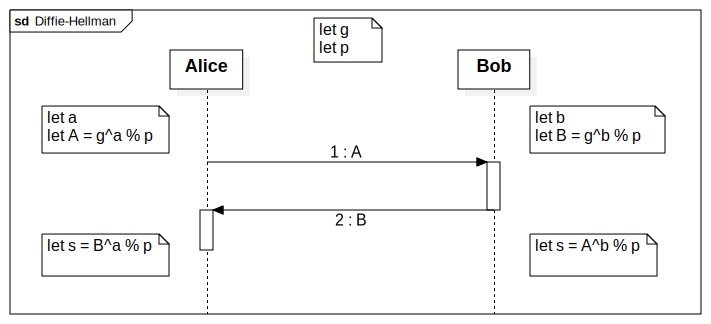
\includegraphics[width=0.8\textwidth]{Diffie-Hellman.pdf}
    \caption{Алгоритм обмена ключей Diffie-Hellman}
    \label{fig:dh}
\end{figure}

Рассмотрим подробнее структуры, используемые для этого алгоритма.

\begin{minted}[samepage,linenos]{rust}
struct DHConfig {
    base: u64,
    modulus: u64
}
\end{minted}

В алгоритме используются две общие для всех константы: `base` и `modulus` (`g` и `p` на рисунке \ref{fig:dh} соответственно) --- основание и модуль (модуль должен быть простым числом). `DHConfig` используется для хранения этих констант.

\begin{minted}[samepage,linenos]{rust}
struct DH {
    config: DHConfig,
    private_key: u32
}
\end{minted}

`DH` --- основная структура, определяющая логику алгоритма Diffie-Hellman, хранящая конфигурацию алгоритма и сгенерированный приватный ключ (`a` и `b` на рисунке \ref{fig:dh}). Эта структура позволяет получить публичный ключ, а также приватный ключ.

Публичный ключ при обмене передаётся неявно: как было описано в \ref{ya:users}, `PeerId` состоит из 16 байтов, семь из которых --- со второго по восьмой включительно --- представляют собой 56-битный публичный ключ (то есть `p` --- 56 битовое простое число).

Приватный ключ получается из `DH` и `Peer` пользователя, с которым устанавливается контакт. Так как приватный ключ также имеет длину 56 бит, он на прямую не применим в AES256. В шифровании используется хэш полученного публичного ключа, вычисляемый алгоритмом SHA256.

\subsection{KeyChain}
`KeyChain` --- блокчейн без хранения всей цепи ключей. Простой, но эффективный способ обновления ключа шифрования.

\begin{minted}[samepage,linenos]{rust}
struct KeyChain {
    top: Mutex<[u8; 32]>
}    
\end{minted}

Новый ключ строится как хэш от предыдущего ключа и переданного нового ключа (32-байтного блока). 

Таким образом, ключ шифрования постоянно обновляется. Кроме того, злоумышленнику для взлома сообщения необходимо хранить всю цепь сообщений с момента удачного взлома.
